The segmentation of the pelvis was evaluated with Dice similarity coefficient given by the formula:
\begin{equation}
	\label{eq:dice}
	DS = \dfrac{2|A}{•},
\end{equation}
where $||x_i-c_j||$ is  the Euclidean distance between a data point $x_i$ and the cluster centre $c_j$ of k predefined clusters. 
The segmentation of the pelvis obtained for the sample kidney is shown on the Figure \ref{fig:kidney_segmented}. 

The example of the time concentration curves after baseline removal for the kidney and aorta are shown on Figure \ref{fig:removed_baseline}. 

Fitting of the time course for different pharmacokinetic models  is illustreted on the Figure~\ref{fig:models}.



\begin{figure*}[h!]
	\centering
	\subfloat[Segmented kidney]{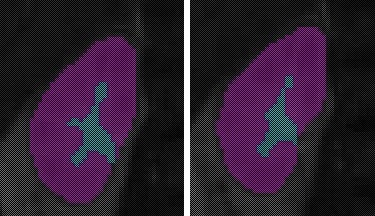
\includegraphics[height=4 cm]{img/kidney_pelvis}}\quad
	\subfloat[Parenchymal volume]{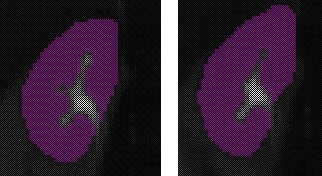
\includegraphics[height=4 cm]{img/no_pelvis}}\\	
	\caption{The sample segmented kidney (a) and parenchymal volume with removed pelvis (b) purple - renal parenchyma, blue - renal pelvis.}
\label{fig:kidney_segmented}
\end{figure*}


\begin{figure*}[h!]
	\centering
	\subfloat[Kidney time course]{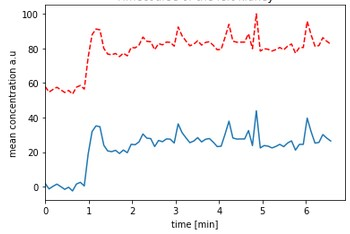
\includegraphics[width=7 cm]{img/kidney_no_baseline}}\quad
	\subfloat[Aorta time course]{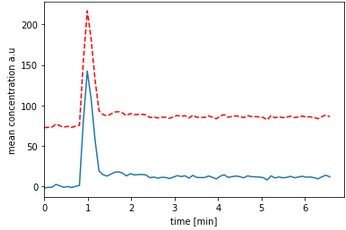
\includegraphics[width=7 cm]{img/aorta_no_baseline}}\\	
\caption{Sample average time-concentration curves for renal parenchyma (a) and aorta (b). The red curve shows the original data while the blue one - after baseline removal.}
\label{fig:removed_baseline}
\end{figure*}

\begin{figure*}[h!]
	\centering
	\subfloat[Toft's model]{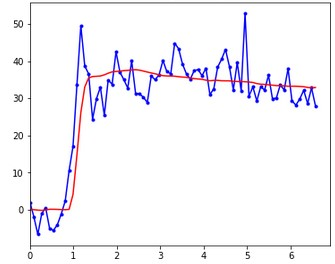
\includegraphics[width=4.5 cm]{img/tk}}\quad
	\subfloat[Extended Toft's model]{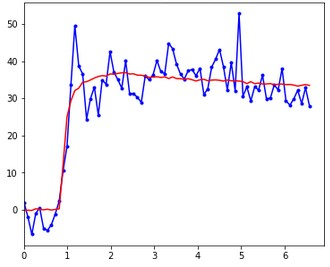
\includegraphics[width=4.5 cm]{img/etk}}\quad
	\subfloat[Patlak model]{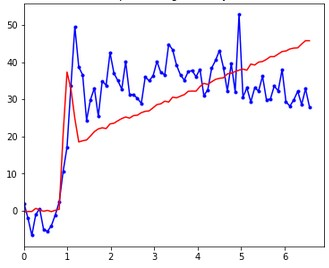
\includegraphics[width=4.5 cm]{img/patlak}}\\	
\caption{Fit of the time-concentration curve of sample kidney to three different PK models.}
\label{fig:models}
\end{figure*}

\newpage

